%============================================================
% MTH 112 Project - Complex numbers
% Updated 202504
%============================================================

\section{Complex Numbers} \label{section-complex-numbers}
In this section, we will learn about complex numbers. We will learn how to plot complex numbers in the complex plane, convert complex numbers between polar, rectangular, and Euler forms, and how to arithmetic with complex numbers.

\textbooks{\href{https://openstax.org/books/algebra-and-trigonometry-2e/pages/10-5-polar-form-of-complex-numbers}{10.5}}{\href{https://openstax.org/books/algebra-and-trigonometry-2e/pages/2-4-complex-numbers}{2.4}}

\subsection*{Preparation Exercises} \label{preparation-exercises-section-complex-numbers}

Answer the following. These questions are intended to check the prerequisite skills needed to complete the rest of the lab.

\begin{myPrep}
	Convert the polar point $\left(4,\frac{7\pi}{6}\right)_p$ to rectangular form. Leave your components in exact form.
\end{myPrep}
\vfill

\begin{myPrep}
	Convert the rectangular point $(-5,2)_r$ to polar form. Use your calculator to find an angle in radians rounded to two digits behind the decimal place.
\end{myPrep}
\vfill

\begin{myPrep}
	\begin{multicols}{2}
		For the right triangle shown in Figure \ref{section-complex-numbers-triangle-solving}, find the missing length of $r$ and the missing angle $\theta$ using SOHCAHTOA. You can use a calculator to help get an approximation, accurate to 4 digits behind the decimal place.
			\columnbreak
			\begin{center}\captionsetup{type=figure} \captionof{figure}{A right triangle}
				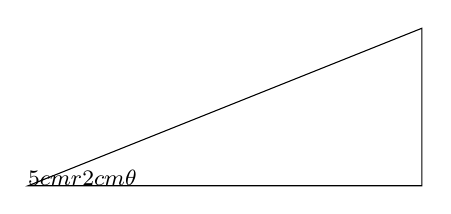
\begin{tikzpicture}[thin] \label{section-complex-numbers-triangle-solving}
					\coordinate (O) at (0,0);
					\coordinate (A) at (5,0);
					\coordinate (B) at (5,2);
					\draw (O)--(A)--(B)--cycle;
					\footnotesize
					\tkzLabelSegment[below=2pt](O,A){$5\text{cm}$}
					\tkzLabelSegment[above=2pt](O,B){$r$}
					\tkzLabelSegment[right=2pt](A,B){$2\text{cm}$}
					\tkzMarkRightAngle[size=0.5](B,A,O)
					\tkzMarkAngle[size=1.3cm](A,O,B)
					\tkzLabelAngle[pos = 1](A,O,B){$\theta$}
				\end{tikzpicture}
			\end{center}
	\end{multicols}
\end{myPrep}
\vfill
\vfill

%======================================================
\newpage
%======================================================

\subsection*{Practice Exercises} \label{practice-exercises-section-complex-numbers}

\begin{myPractice}
		\begin{multicols}{2}
			Plot the complex numbers onto Figure \ref{section-complex-numbers-practice-plotting}.
				\begin{enumerate}[itemsep=.5cm]
					\item $2+3i$
					\item $-1+2i$
					\item $-3i$
					\item $3-i$
				\end{enumerate}
				\columnbreak
				\begin{center}\captionsetup{type=figure} \captionof{figure}{A complex plane}
					\begin{tikzpicture}[thin] \label{section-complex-numbers-practice-plotting}
 						\begin{axis}[
 							height=6cm,
 							width=6cm,
 							framed,
 							ylabel={$y_i$},
 							xmin=-4,xmax=4,
 							ymin=-4,ymax=4,
						    xtick={-3,-2,...,3},
						    ytick={-3,-2,...,3},
						    grid=both,
 							]
 						\end{axis}
					\end{tikzpicture}
				\end{center}
		\end{multicols}
\end{myPractice}

\begin{myPractice}
		Find the absolute value and argument of the complex numbers.
			\begin{enumerate}
				\begin{multicols}{2}
					\item $2+3i$
					\item $-1+2i$
				\end{multicols}
			\end{enumerate}
		\vfill
\end{myPractice}

\begin{myPractice}
	\begin{enumerate}
		\item Convert the standard form complex number $5-12i$ into polar form. Use radians and round your argument to two digits behind the decimal place.
		\vfill
		\item Convert the polar form complex number $7\left(\cos\left(\frac{5\pi}{6}\right)+i\sin\left(\frac{5\pi}{6}\right)\right)$ into standard form. Keep your values exact using your memorized values on the unit circle.
		\vfill
	\end{enumerate}
\end{myPractice}

%======================================================
\newpage
%======================================================

\begin{myPractice}
	Simplify the expressions completely.
	\begin{enumerate}[itemsep=3cm]
		\begin{multicols}{2}
			\item $(2i)^4$
			\item $(2i+3)-(4i-1)$
			\columnbreak
			\item $(2i+3)\cdot(4i-1)$
		\end{multicols}
	\end{enumerate}
\end{myPractice}
\vfill

\begin{myPractice}
	\begin{enumerate}
		\item Convert the standard form complex number $5-12i$ into Euler's form. Use radians and round your argument to two digits behind the decimal place.
		\vfill
		\item Convert the Euler's form complex number $7e^{\frac{4\pi i}{3}}$ into standard form. Keep your values exact using your memorized values on the unit circle.
		\vfill
	\end{enumerate}
\end{myPractice}

%======================================================
\newpage
%======================================================

\subsection*{Definitions} \label{definitions-section-complex-numbers}

\begin{myDefinition}[The Imaginary unit $i$]
The \textbf{imaginary unit $i$} is defined to be $i=\sqrt{-1}$. Since there is no real number that is multiplied by itself to create a negative number, $i$ must not be a real number. It fits into a new category of numbers called imaginary numbers which are any multiples of $i$. It's called a \say{unit} because its absolute value is $1$.
\newline For example, $4i$, $-2i$, and $\sqrt{-9}$ are all imaginary numbers.
\end{myDefinition}

\begin{myDefinition}[{Standard form of a Complex Number}]~\\[0.5mm]
A \textbf{complex number} is any real number plus any imaginary number. Any complex number can be written in standard form (also called rectangular form), which is the form $a+bi$, where both $a$ and $b$ are real numbers. 
\newline For example, $3+0i$, $0-2i$, and $1-\sqrt{5}i$ are all complex numbers.
\end{myDefinition}

\begin{myDefinition}[{The Complex plane}]~\\[0.5mm]
The \textbf{complex plane} is the two dimensional axes system to plot complex numbers. The horizontal axis, often just labeled $x$, measures the real part of a complex number. The vertical axis, often labeled $y_i$, measures the imaginary part of a complex number. 
\newline For example, the number $-3+4i$ would be plotted $3$ units to the left and $4$ units up from the origin at the same place that $(-3,4)$ would have been plotted in the regular two-dimensional real axes.
\end{myDefinition}

\begin{myDefinition}[{Absolute Value of a Complex number}]~\\[0.5mm]
The \textbf{absolute value of the complex number} is the distance from the origin to the number in the complex plane. The absolute value is written as usual, $\abs{z}$. To find the absolute value of $z=a+bi$, use the Pythagorean Theorem: $\abs{z}=\sqrt{a^2+b^2}$. 
\newline \emph{Note}: the $i$ is \emph{dropped} during this calculation! 
\newline \emph{Note}: the absolute value of a complex number is sometimes also called the magnitude or modulus.
\newline For Example, to find the absolute value of $z=-3+4i$, we would write that $\abs{z}=\sqrt{(-3)^2+4^2}=5$. 
\end{myDefinition}

\begin{multicols}{2}
	\begin{myDefinition}[{Argument of a Complex number}]~\\[0.5mm]
	The \textbf{argument of the complex number}, $z=a+bi$, is an angle, $\theta$ measured from the standard position to the number in the complex plane. To find this angle, $\theta$, use the formula $\tan(\theta)=\frac{b}{a}$ and solve for $\theta$ that is in the correct quadrant. 
	\newline \emph{Note}: the $i$ is \emph{dropped} during this calculation! 
	\newline For example, to find the argument of $z=-3+4i$, we would first note that $z$ is in the second quadrant, and we would write $\tan(\theta)=\frac{4}{-3}$. Next, we would take the inverse-tangent on both sides, \emph{however}, inverse-tangent does not give us angles in quadrant II, so we know that to find the correct argument of $z$ we should add $\pi$. So the argument of $z$ is $\theta=\tan^{-1}\left(\frac{4}{-3}\right)+\pi\approx2.21$, as shown in Figure \ref{section-complex-numbers-abs-val-and-argument}.
	\end{myDefinition}

	\begin{center}\captionsetup{type=figure} \captionof{figure}{A graph of $z=-3+4i$ showing the absolute value and argument of $z$}
		\begin{tikzpicture}[thin] \label{section-complex-numbers-abs-val-and-argument}
 			\begin{axis}[
 				framed,
 				ylabel={$y_i$},
 				xmin=-4,xmax=2,
 				ymin=-1,ymax=5,
			    xtick={-3,-2,-1,1},
			    ytick={1,2,3,4},
			    grid=both,
 				]
 				\draw 	(-3,4) node[above,color=first] {$-3+4i$};
 				\draw 	(1,1.3) node[color=third] {$\theta\approx2.21$};
				\addplot[only marks, mark=*,color=first] coordinates{(-3,4)(0,0)};
				\addplot[dashed,color=second,thin] coordinates{(-3,4)(0,0)};
				\addplot[domain= 0:126.87,third] ({cos(x)},{sin(x)});
				\draw 	(-1.5,2) node[above,color=second,rotate=-atan(4/3)] {$\abs{z}=5$};
 			\end{axis}
		\end{tikzpicture}
	\end{center}
\end{multicols}

\begin{myDefinition}[{Polar form of a Complex number}]~\\[0.5mm]
A complex number can be written in \textbf{polar form}, which is the form $r\left(\cos(\theta)+i\sin(\theta)\right)$, where $r=\abs{z}$ and and $\theta$ is the argument of the complex number. 
\newline For example, $z=-3+4i$ can be written as $z\approx5\left(\cos(2.21)+i\sin(2.21)\right)$. 
\newline \emph{Note}: We used the $\approx$ symbol here because the $2.21$ was an approximate value. 
\newline \emph{Note}: $\cos(\theta)+i\sin(\theta)$ is sometimes called $\text{cis}(\theta)$.
\end{myDefinition}

\begin{myDefinition}[{Euler's form of a Complex number}]~\\[0.5mm]
\textbf{Euler's form} of a complex number, $z$, is $z=re^{i\theta}$, where $r=\abs{z}$ and $\theta$ is the argument of $z$. 
\newline For example, $z=-3+4i$ can be written as $z\approx5e^{i\cdot2.21}$. 
\newline \emph{Note}: We used the $\approx$ symbol here because the $2.21$ was an approximate value.
\end{myDefinition}

%======================================================
\newpage
%======================================================

\subsection*{Exit Exercises} \label{exit-exercises-section-complex-numbers}

\begin{myExit}
	Describe the difference between the point $(5,8)$ in the two-dimensional real coordinate plane and the complex number $5+8i$ in the complex plane.
\end{myExit}

\begin{myExit}
	\begin{enumerate}
		\begin{multicols}{2}
			\item Plot the complex number $-6-4i$ onto Figure \ref{section-complex-numbers-exit-plotting}.
			\item Find the absolute value of the complex number $-6-4i$. Simplify the radical completely and leave your answer in exact form. Illustrate this value on Figure \ref{section-complex-numbers-exit-plotting}.
			\vfill
			\item Find the argument of the complex number \newline$-6-4i$. Use a calculator to round your answer to three digits behind the decimal place. Illustrate this value on Figure \ref{section-complex-numbers-exit-plotting}.
			\vfill
			\columnbreak
			\begin{center}\captionsetup{type=figure} \captionof{figure}{A complex plane to plot complex numbers}
				\begin{tikzpicture}[thin] \label{section-complex-numbers-exit-plotting}
 					\begin{axis}[
 						framed,
 						ylabel={$y_i$},
 						xmin=-7,xmax=7,
 						ymin=-7,ymax=7,
					    xtick={-6,-5,...,6},
					    ytick={-6,-5,...,6},
					    grid=both,
 						]
 					\end{axis}
				\end{tikzpicture}
			\end{center}
		\end{multicols}
	\end{enumerate}
	\begin{enumerate}\setcounter{enumi}{3}
		\vfill
		\item Write the complex number $-6-4i$ into polar form. 
		\vfill
		\item Write the complex number $-6-4i$ into Euler's form. 
		\vfill
	\end{enumerate}
\end{myExit}
\exitlikert{complex numbers}